\documentclass[1p]{elsarticle_modified}
%\bibliographystyle{elsarticle-num}

%\usepackage[colorlinks]{hyperref}
%\usepackage{abbrmath_seonhwa} %\Abb, \Ascr, \Acal ,\Abf, \Afrak
\usepackage{amsfonts}
\usepackage{amssymb}
\usepackage{amsmath}
\usepackage{amsthm}
\usepackage{scalefnt}
\usepackage{amsbsy}
\usepackage{kotex}
\usepackage{caption}
\usepackage{subfig}
\usepackage{color}
\usepackage{graphicx}
\usepackage{xcolor} %% white, black, red, green, blue, cyan, magenta, yellow
\usepackage{float}
\usepackage{setspace}
\usepackage{hyperref}

\usepackage{tikz}
\usetikzlibrary{arrows}

\usepackage{multirow}
\usepackage{array} % fixed length table
\usepackage{hhline}

%%%%%%%%%%%%%%%%%%%%%
\makeatletter
\renewcommand*\env@matrix[1][\arraystretch]{%
	\edef\arraystretch{#1}%
	\hskip -\arraycolsep
	\let\@ifnextchar\new@ifnextchar
	\array{*\c@MaxMatrixCols c}}
\makeatother %https://tex.stackexchange.com/questions/14071/how-can-i-increase-the-line-spacing-in-a-matrix
%%%%%%%%%%%%%%%

\usepackage[normalem]{ulem}

\newcommand{\msout}[1]{\ifmmode\text{\sout{\ensuremath{#1}}}\else\sout{#1}\fi}
%SOURCE: \msout is \stkout macro in https://tex.stackexchange.com/questions/20609/strikeout-in-math-mode

\newcommand{\cancel}[1]{
	\ifmmode
	{\color{red}\msout{#1}}
	\else
	{\color{red}\sout{#1}}
	\fi
}

\newcommand{\add}[1]{
	{\color{blue}\uwave{#1}}
}

\newcommand{\replace}[2]{
	\ifmmode
	{\color{red}\msout{#1}}{\color{blue}\uwave{#2}}
	\else
	{\color{red}\sout{#1}}{\color{blue}\uwave{#2}}
	\fi
}

\newcommand{\Sol}{\mathcal{S}} %segment
\newcommand{\D}{D} %diagram
\newcommand{\A}{\mathcal{A}} %arc


%%%%%%%%%%%%%%%%%%%%%%%%%%%%%5 test

\def\sl{\operatorname{\textup{SL}}(2,\Cbb)}
\def\psl{\operatorname{\textup{PSL}}(2,\Cbb)}
\def\quan{\mkern 1mu \triangleright \mkern 1mu}

\theoremstyle{definition}
\newtheorem{thm}{Theorem}[section]
\newtheorem{prop}[thm]{Proposition}
\newtheorem{lem}[thm]{Lemma}
\newtheorem{ques}[thm]{Question}
\newtheorem{cor}[thm]{Corollary}
\newtheorem{defn}[thm]{Definition}
\newtheorem{exam}[thm]{Example}
\newtheorem{rmk}[thm]{Remark}
\newtheorem{alg}[thm]{Algorithm}

\newcommand{\I}{\sqrt{-1}}
\begin{document}

%\begin{frontmatter}
%
%\title{Boundary parabolic representations of knots up to 8 crossings}
%
%%% Group authors per affiliation:
%\author{Yunhi Cho} 
%\address{Department of Mathematics, University of Seoul, Seoul, Korea}
%\ead{yhcho@uos.ac.kr}
%
%
%\author{Seonhwa Kim} %\fnref{s_kim}}
%\address{Center for Geometry and Physics, Institute for Basic Science, Pohang, 37673, Korea}
%\ead{ryeona17@ibs.re.kr}
%
%\author{Hyuk Kim}
%\address{Department of Mathematical Sciences, Seoul National University, Seoul 08826, Korea}
%\ead{hyukkim@snu.ac.kr}
%
%\author{Seokbeom Yoon}
%\address{Department of Mathematical Sciences, Seoul National University, Seoul, 08826,  Korea}
%\ead{sbyoon15@snu.ac.kr}
%
%\begin{abstract}
%We find all boundary parabolic representation of knots up to 8 crossings.
%
%\end{abstract}
%\begin{keyword}
%    \MSC[2010] 57M25 
%\end{keyword}
%
%\end{frontmatter}

%\linenumbers
%\tableofcontents
%
\newcommand\colored[1]{\textcolor{white}{\rule[-0.35ex]{0.8em}{1.4ex}}\kern-0.8em\color{red} #1}%
%\newcommand\colored[1]{\textcolor{white}{ #1}\kern-2.17ex	\textcolor{white}{ #1}\kern-1.81ex	\textcolor{white}{ #1}\kern-2.15ex\color{red}#1	}

{\Large $\underline{12n_{0278}~(K12n_{0278})}$}

\setlength{\tabcolsep}{10pt}
\renewcommand{\arraystretch}{1.6}
\vspace{1cm}\begin{tabular}{m{100pt}>{\centering\arraybackslash}m{274pt}}
\multirow{5}{120pt}{
	\centering
	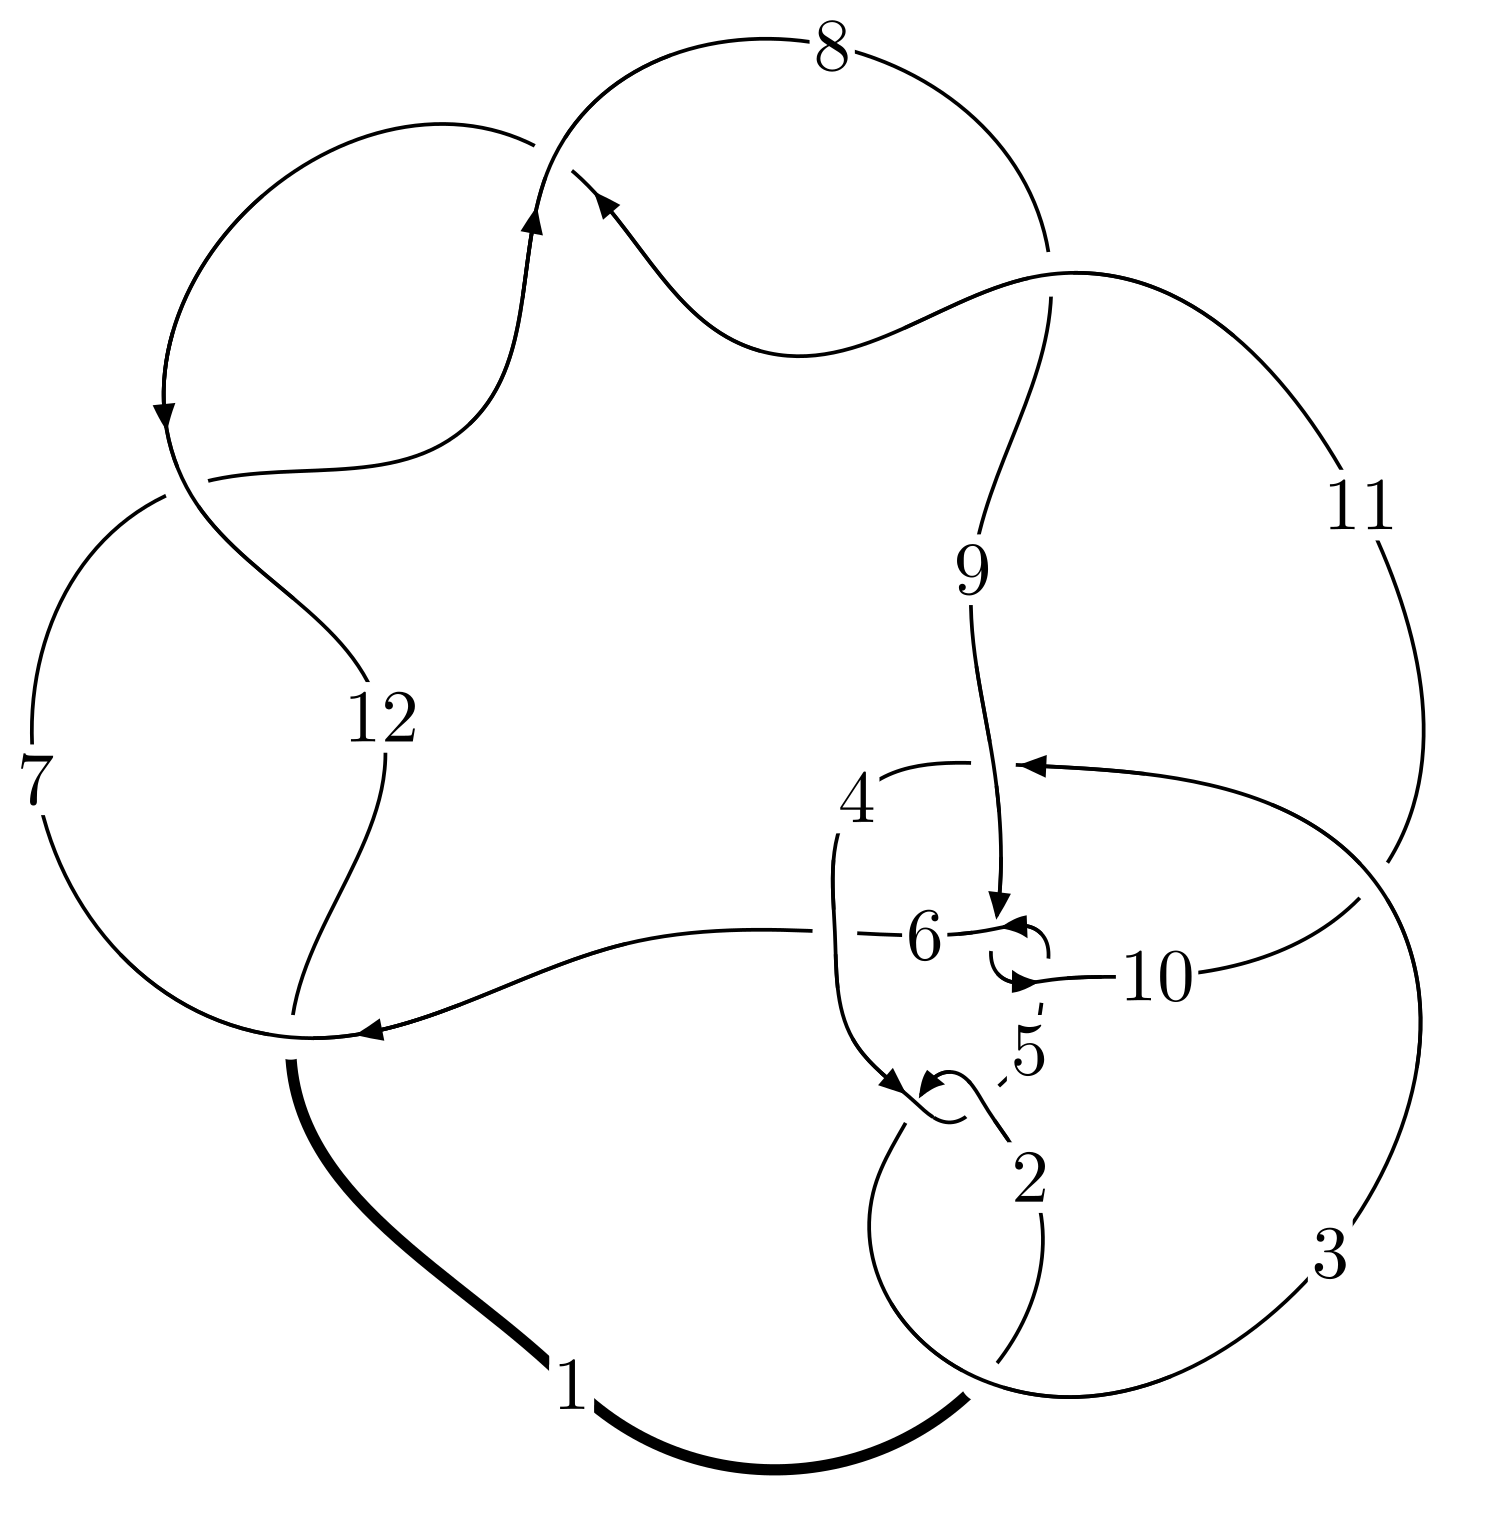
\includegraphics[width=112pt]{../../../GIT/diagram.site/Diagrams/png/2367_12n_0278.png}\\
\ \ \ A knot diagram\footnotemark}&
\allowdisplaybreaks
\textbf{Linearized knot diagam} \\
\cline{2-2}
 &
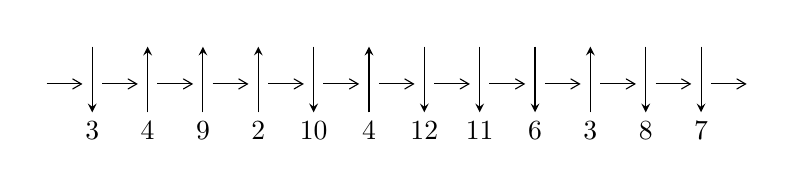
\begin{tikzpicture}[x=20pt, y=17pt]
	% nodes
	\node (C0) at (0, 0) {};
	\node (C1) at (1, 0) {};
	\node (C1U) at (1, +1) {};
	\node (C1D) at (1, -1) {3};

	\node (C2) at (2, 0) {};
	\node (C2U) at (2, +1) {};
	\node (C2D) at (2, -1) {4};

	\node (C3) at (3, 0) {};
	\node (C3U) at (3, +1) {};
	\node (C3D) at (3, -1) {9};

	\node (C4) at (4, 0) {};
	\node (C4U) at (4, +1) {};
	\node (C4D) at (4, -1) {2};

	\node (C5) at (5, 0) {};
	\node (C5U) at (5, +1) {};
	\node (C5D) at (5, -1) {10};

	\node (C6) at (6, 0) {};
	\node (C6U) at (6, +1) {};
	\node (C6D) at (6, -1) {4};

	\node (C7) at (7, 0) {};
	\node (C7U) at (7, +1) {};
	\node (C7D) at (7, -1) {12};

	\node (C8) at (8, 0) {};
	\node (C8U) at (8, +1) {};
	\node (C8D) at (8, -1) {11};

	\node (C9) at (9, 0) {};
	\node (C9U) at (9, +1) {};
	\node (C9D) at (9, -1) {6};

	\node (C10) at (10, 0) {};
	\node (C10U) at (10, +1) {};
	\node (C10D) at (10, -1) {3};

	\node (C11) at (11, 0) {};
	\node (C11U) at (11, +1) {};
	\node (C11D) at (11, -1) {8};

	\node (C12) at (12, 0) {};
	\node (C12U) at (12, +1) {};
	\node (C12D) at (12, -1) {7};
	\node (C13) at (13, 0) {};

	% arrows
	\draw[->,>={angle 60}]
	(C0) edge (C1) (C1) edge (C2) (C2) edge (C3) (C3) edge (C4) (C4) edge (C5) (C5) edge (C6) (C6) edge (C7) (C7) edge (C8) (C8) edge (C9) (C9) edge (C10) (C10) edge (C11) (C11) edge (C12) (C12) edge (C13) ;	\draw[->,>=stealth]
	(C1U) edge (C1D) (C2D) edge (C2U) (C3D) edge (C3U) (C4D) edge (C4U) (C5U) edge (C5D) (C6D) edge (C6U) (C7U) edge (C7D) (C8U) edge (C8D) (C9U) edge (C9D) (C10D) edge (C10U) (C11U) edge (C11D) (C12U) edge (C12D) ;
	\end{tikzpicture} \\
\hhline{~~} \\& 
\textbf{Solving Sequence} \\ \cline{2-2} 
 &
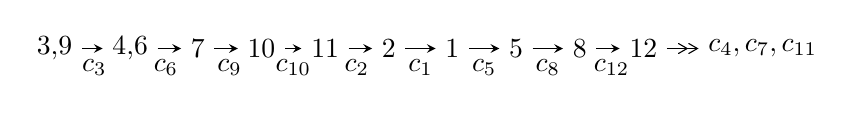
\begin{tikzpicture}[x=23pt, y=7pt]
	% node
	\node (A0) at (-1/8, 0) {3,9};
	\node (A1) at (17/16, 0) {4,6};
	\node (A2) at (17/8, 0) {7};
	\node (A3) at (25/8, 0) {10};
	\node (A4) at (33/8, 0) {11};
	\node (A5) at (41/8, 0) {2};
	\node (A6) at (49/8, 0) {1};
	\node (A7) at (57/8, 0) {5};
	\node (A8) at (65/8, 0) {8};
	\node (A9) at (73/8, 0) {12};
	\node (C1) at (1/2, -1) {$c_{3}$};
	\node (C2) at (13/8, -1) {$c_{6}$};
	\node (C3) at (21/8, -1) {$c_{9}$};
	\node (C4) at (29/8, -1) {$c_{10}$};
	\node (C5) at (37/8, -1) {$c_{2}$};
	\node (C6) at (45/8, -1) {$c_{1}$};
	\node (C7) at (53/8, -1) {$c_{5}$};
	\node (C8) at (61/8, -1) {$c_{8}$};
	\node (C9) at (69/8, -1) {$c_{12}$};
	\node (A10) at (11, 0) {$c_{4},c_{7},c_{11}$};

	% edge
	\draw[->,>=stealth]	
	(A0) edge (A1) (A1) edge (A2) (A2) edge (A3) (A3) edge (A4) (A4) edge (A5) (A5) edge (A6) (A6) edge (A7) (A7) edge (A8) (A8) edge (A9) ;
	\draw[->>,>={angle 60}]	
	(A9) edge (A10);
\end{tikzpicture} \\ 

\end{tabular} \\

\footnotetext{
The image of knot diagram is generated by the software ``\textbf{Draw programme}" developed by Andrew Bartholomew(\url{http://www.layer8.co.uk/maths/draw/index.htm\#Running-draw}), where we modified some parts for our purpose(\url{https://github.com/CATsTAILs/LinksPainter}).
}\phantom \\ \newline 
\centering \textbf{Ideals for irreducible components\footnotemark of $X_{\text{par}}$} 
 
\begin{align*}
I^u_{1}&=\langle 
-635380494822630 u^{39}-689616041260383 u^{38}+\cdots+1433600017911488 b+1677666964673313,\\
\phantom{I^u_{1}}&\phantom{= \langle  }2246684406994641 u^{39}+1078394006282716 u^{38}+\cdots+7168000089557440 a+9725037800310384,\\
\phantom{I^u_{1}}&\phantom{= \langle  }u^{40}+u^{39}+\cdots+4 u+5\rangle \\
I^u_{2}&=\langle 
u^3 b+4 u^2 b- u^3+b^2- b u+u^2-2 b- u-4,\;- u^2+a,\;u^4- u^2+1\rangle \\
\\
\end{align*}
\raggedright * 2 irreducible components of $\dim_{\mathbb{C}}=0$, with total 48 representations.\\
\footnotetext{All coefficients of polynomials are rational numbers. But the coefficients are sometimes approximated in decimal forms when there is not enough margin.}
\newpage
\renewcommand{\arraystretch}{1}
\centering \section*{I. $I^u_{1}= \langle -6.35\times10^{14} u^{39}-6.90\times10^{14} u^{38}+\cdots+1.43\times10^{15} b+1.68\times10^{15},\;2.25\times10^{15} u^{39}+1.08\times10^{15} u^{38}+\cdots+7.17\times10^{15} a+9.73\times10^{15},\;u^{40}+u^{39}+\cdots+4 u+5 \rangle$}
\flushleft \textbf{(i) Arc colorings}\\
\begin{tabular}{m{7pt} m{180pt} m{7pt} m{180pt} }
\flushright $a_{3}=$&$\begin{pmatrix}1\\0\end{pmatrix}$ \\
\flushright $a_{9}=$&$\begin{pmatrix}0\\u\end{pmatrix}$ \\
\flushright $a_{4}=$&$\begin{pmatrix}1\\- u^2\end{pmatrix}$ \\
\flushright $a_{6}=$&$\begin{pmatrix}-0.313433 u^{39}-0.150446 u^{38}+\cdots+1.82893 u-1.35673\\0.443206 u^{39}+0.481038 u^{38}+\cdots-5.21478 u-1.17025\end{pmatrix}$ \\
\flushright $a_{7}=$&$\begin{pmatrix}-0.109699 u^{39}+0.157341 u^{38}+\cdots-2.47064 u-3.34191\\0.331526 u^{39}+0.441625 u^{38}+\cdots-3.77990 u-0.649983\end{pmatrix}$ \\
\flushright $a_{10}=$&$\begin{pmatrix}-0.286938 u^{39}-0.370199 u^{38}+\cdots+5.00815 u+1.05379\\0.190141 u^{39}-0.0380655 u^{38}+\cdots-2.69477 u+1.78981\end{pmatrix}$ \\
\flushright $a_{11}=$&$\begin{pmatrix}-0.0967963 u^{39}-0.408265 u^{38}+\cdots+2.31338 u+2.84360\\0.190141 u^{39}-0.0380655 u^{38}+\cdots-2.69477 u+1.78981\end{pmatrix}$ \\
\flushright $a_{2}=$&$\begin{pmatrix}- u^2+1\\u^4\end{pmatrix}$ \\
\flushright $a_{1}=$&$\begin{pmatrix}u^4- u^2+1\\u^4\end{pmatrix}$ \\
\flushright $a_{5}=$&$\begin{pmatrix}u^4- u^2+1\\- u^6- u^2\end{pmatrix}$ \\
\flushright $a_{8}=$&$\begin{pmatrix}0.332958 u^{39}+0.469712 u^{38}+\cdots-6.44378 u-1.37541\\0.255919 u^{39}+0.714505 u^{38}+\cdots-6.65923 u-4.34499\end{pmatrix}$ \\
\flushright $a_{12}=$&$\begin{pmatrix}0.453947 u^{39}+0.662238 u^{38}+\cdots-5.70833 u-2.30072\\-0.0932185 u^{39}-0.0614314 u^{38}+\cdots+0.780423 u+1.26772\end{pmatrix}$\\&\end{tabular}
\flushleft \textbf{(ii) Obstruction class $= -1$}\\~\\
\flushleft \textbf{(iii) Cusp Shapes $= -\frac{10623651294159}{102400001279392} u^{39}-\frac{45699572803011}{102400001279392} u^{38}+\cdots+\frac{228874377951323}{25600000319848} u+\frac{930610235166537}{102400001279392}$}\\~\\
\newpage\renewcommand{\arraystretch}{1}
\flushleft \textbf{(iv) u-Polynomials at the component}\newline \\
\begin{tabular}{m{50pt}|m{274pt}}
Crossings & \hspace{64pt}u-Polynomials at each crossing \\
\hline $$\begin{aligned}c_{1}\end{aligned}$$&$\begin{aligned}
&u^{40}+41 u^{39}+\cdots-4756 u+625
\end{aligned}$\\
\hline $$\begin{aligned}c_{2},c_{4}\end{aligned}$$&$\begin{aligned}
&u^{40}-11 u^{39}+\cdots-216 u+25
\end{aligned}$\\
\hline $$\begin{aligned}c_{3}\end{aligned}$$&$\begin{aligned}
&u^{40}+u^{39}+\cdots+4 u+5
\end{aligned}$\\
\hline $$\begin{aligned}c_{5},c_{9}\end{aligned}$$&$\begin{aligned}
&u^{40}+u^{39}+\cdots+13 u^2+4
\end{aligned}$\\
\hline $$\begin{aligned}c_{6}\end{aligned}$$&$\begin{aligned}
&u^{40}+5 u^{39}+\cdots-11820 u+18731
\end{aligned}$\\
\hline $$\begin{aligned}c_{7},c_{8},c_{11}\\c_{12}\end{aligned}$$&$\begin{aligned}
&u^{40}- u^{39}+\cdots-8 u+1
\end{aligned}$\\
\hline $$\begin{aligned}c_{10}\end{aligned}$$&$\begin{aligned}
&u^{40}-3 u^{39}+\cdots+1600 u+1984
\end{aligned}$\\
\hline
\end{tabular}\\~\\
\newpage\renewcommand{\arraystretch}{1}
\flushleft \textbf{(v) Riley Polynomials at the component}\newline \\
\begin{tabular}{m{50pt}|m{274pt}}
Crossings & \hspace{64pt}Riley Polynomials at each crossing \\
\hline $$\begin{aligned}c_{1}\end{aligned}$$&$\begin{aligned}
&y^{40}-79 y^{39}+\cdots+16952964 y+390625
\end{aligned}$\\
\hline $$\begin{aligned}c_{2},c_{4}\end{aligned}$$&$\begin{aligned}
&y^{40}+41 y^{39}+\cdots-4756 y+625
\end{aligned}$\\
\hline $$\begin{aligned}c_{3}\end{aligned}$$&$\begin{aligned}
&y^{40}-11 y^{39}+\cdots-216 y+25
\end{aligned}$\\
\hline $$\begin{aligned}c_{5},c_{9}\end{aligned}$$&$\begin{aligned}
&y^{40}+13 y^{39}+\cdots+104 y+16
\end{aligned}$\\
\hline $$\begin{aligned}c_{6}\end{aligned}$$&$\begin{aligned}
&y^{40}+31 y^{39}+\cdots+6061334998 y+350850361
\end{aligned}$\\
\hline $$\begin{aligned}c_{7},c_{8},c_{11}\\c_{12}\end{aligned}$$&$\begin{aligned}
&y^{40}+45 y^{39}+\cdots-4 y+1
\end{aligned}$\\
\hline $$\begin{aligned}c_{10}\end{aligned}$$&$\begin{aligned}
&y^{40}+15 y^{39}+\cdots+108480512 y+3936256
\end{aligned}$\\
\hline
\end{tabular}\\~\\
\newpage\flushleft \textbf{(vi) Complex Volumes and Cusp Shapes}
$$\begin{array}{c|c|c}  
\text{Solutions to }I^u_{1}& \I (\text{vol} + \sqrt{-1}CS) & \text{Cusp shape}\\
 \hline 
\begin{aligned}
u &= -0.816138 + 0.601846 I \\
a &= -0.100989 + 0.484046 I \\
b &= \phantom{-}1.272200 + 0.371404 I\end{aligned}
 & \phantom{-}9.03582 - 2.34742 I & -1.16092 + 4.21084 I \\ \hline\begin{aligned}
u &= -0.816138 - 0.601846 I \\
a &= -0.100989 - 0.484046 I \\
b &= \phantom{-}1.272200 - 0.371404 I\end{aligned}
 & \phantom{-}9.03582 + 2.34742 I & -1.16092 - 4.21084 I \\ \hline\begin{aligned}
u &= \phantom{-}0.942774 + 0.425003 I \\
a &= \phantom{-}0.249731 + 0.561680 I \\
b &= \phantom{-}0.05704 - 1.50077 I\end{aligned}
 & \phantom{-}1.43856 + 1.71130 I & -1.298482 + 0.550005 I \\ \hline\begin{aligned}
u &= \phantom{-}0.942774 - 0.425003 I \\
a &= \phantom{-}0.249731 - 0.561680 I \\
b &= \phantom{-}0.05704 + 1.50077 I\end{aligned}
 & \phantom{-}1.43856 - 1.71130 I & -1.298482 - 0.550005 I \\ \hline\begin{aligned}
u &= \phantom{-}0.778485 + 0.532883 I \\
a &= \phantom{-}0.574413 + 1.007710 I \\
b &= \phantom{-}0.08684 - 1.66241 I\end{aligned}
 & \phantom{-}1.51229 + 2.11244 I & -4.00016 - 4.74712 I \\ \hline\begin{aligned}
u &= \phantom{-}0.778485 - 0.532883 I \\
a &= \phantom{-}0.574413 - 1.007710 I \\
b &= \phantom{-}0.08684 + 1.66241 I\end{aligned}
 & \phantom{-}1.51229 - 2.11244 I & -4.00016 + 4.74712 I \\ \hline\begin{aligned}
u &= -1.044590 + 0.339980 I \\
a &= -0.206550 - 0.804001 I \\
b &= \phantom{-}0.54339 + 2.06103 I\end{aligned}
 & \phantom{-}1.66475 - 4.28233 I & \phantom{-}1.04865 + 9.16728 I \\ \hline\begin{aligned}
u &= -1.044590 - 0.339980 I \\
a &= -0.206550 + 0.804001 I \\
b &= \phantom{-}0.54339 - 2.06103 I\end{aligned}
 & \phantom{-}1.66475 + 4.28233 I & \phantom{-}1.04865 - 9.16728 I \\ \hline\begin{aligned}
u &= -0.870167 + 0.752444 I \\
a &= \phantom{-}0.817881 - 0.905901 I \\
b &= \phantom{-}0.43266 + 2.06327 I\end{aligned}
 & \phantom{-}6.83536 - 2.84310 I & \phantom{-}2.40205 + 2.94368 I \\ \hline\begin{aligned}
u &= -0.870167 - 0.752444 I \\
a &= \phantom{-}0.817881 + 0.905901 I \\
b &= \phantom{-}0.43266 - 2.06327 I\end{aligned}
 & \phantom{-}6.83536 + 2.84310 I & \phantom{-}2.40205 - 2.94368 I\\
 \hline 
 \end{array}$$\newpage$$\begin{array}{c|c|c}  
\text{Solutions to }I^u_{1}& \I (\text{vol} + \sqrt{-1}CS) & \text{Cusp shape}\\
 \hline 
\begin{aligned}
u &= \phantom{-}0.642627 + 0.538012 I \\
a &= \phantom{-}0.365174 - 0.413262 I \\
b &= \phantom{-}0.325214 - 0.141593 I\end{aligned}
 & \phantom{-}0.58360 + 1.86035 I & -1.76602 - 5.14793 I \\ \hline\begin{aligned}
u &= \phantom{-}0.642627 - 0.538012 I \\
a &= \phantom{-}0.365174 + 0.413262 I \\
b &= \phantom{-}0.325214 + 0.141593 I\end{aligned}
 & \phantom{-}0.58360 - 1.86035 I & -1.76602 + 5.14793 I \\ \hline\begin{aligned}
u &= -1.100630 + 0.389040 I \\
a &= \phantom{-}0.706000 - 0.374232 I \\
b &= -0.84428 + 1.49004 I\end{aligned}
 & \phantom{-}7.52435 - 1.33305 I & \phantom{-}3.41871 + 0.66465 I \\ \hline\begin{aligned}
u &= -1.100630 - 0.389040 I \\
a &= \phantom{-}0.706000 + 0.374232 I \\
b &= -0.84428 - 1.49004 I\end{aligned}
 & \phantom{-}7.52435 + 1.33305 I & \phantom{-}3.41871 - 0.66465 I \\ \hline\begin{aligned}
u &= \phantom{-}1.153370 + 0.265663 I \\
a &= -0.361327 + 0.909523 I \\
b &= \phantom{-}0.80159 - 2.60812 I\end{aligned}
 & \phantom{-}8.28312 + 6.34531 I & \phantom{-}4.99183 - 5.94173 I \\ \hline\begin{aligned}
u &= \phantom{-}1.153370 - 0.265663 I \\
a &= -0.361327 - 0.909523 I \\
b &= \phantom{-}0.80159 + 2.60812 I\end{aligned}
 & \phantom{-}8.28312 - 6.34531 I & \phantom{-}4.99183 + 5.94173 I \\ \hline\begin{aligned}
u &= -0.740318 + 0.931805 I \\
a &= -1.181910 + 0.030020 I \\
b &= -0.522469 - 0.429658 I\end{aligned}
 & \phantom{-}0.02606 + 6.35035 I & \phantom{-}0.13702 - 2.71532 I \\ \hline\begin{aligned}
u &= -0.740318 - 0.931805 I \\
a &= -1.181910 - 0.030020 I \\
b &= -0.522469 + 0.429658 I\end{aligned}
 & \phantom{-}0.02606 - 6.35035 I & \phantom{-}0.13702 + 2.71532 I \\ \hline\begin{aligned}
u &= -0.057006 + 0.799683 I \\
a &= \phantom{-}0.932252 - 0.995287 I \\
b &= \phantom{-}0.476313 + 0.200122 I\end{aligned}
 & \phantom{-}4.23419 - 2.71559 I & -0.50842 + 3.06868 I \\ \hline\begin{aligned}
u &= -0.057006 - 0.799683 I \\
a &= \phantom{-}0.932252 + 0.995287 I \\
b &= \phantom{-}0.476313 - 0.200122 I\end{aligned}
 & \phantom{-}4.23419 + 2.71559 I & -0.50842 - 3.06868 I\\
 \hline 
 \end{array}$$\newpage$$\begin{array}{c|c|c}  
\text{Solutions to }I^u_{1}& \I (\text{vol} + \sqrt{-1}CS) & \text{Cusp shape}\\
 \hline 
\begin{aligned}
u &= \phantom{-}0.846654 + 0.893541 I \\
a &= \phantom{-}0.153750 - 0.996865 I \\
b &= -0.370640 + 1.101610 I\end{aligned}
 & -1.261380 + 0.472950 I & -0.86316 - 1.46415 I \\ \hline\begin{aligned}
u &= \phantom{-}0.846654 - 0.893541 I \\
a &= \phantom{-}0.153750 + 0.996865 I \\
b &= -0.370640 - 1.101610 I\end{aligned}
 & -1.261380 - 0.472950 I & -0.86316 + 1.46415 I \\ \hline\begin{aligned}
u &= \phantom{-}0.824369 + 0.917399 I \\
a &= -1.102340 + 0.038722 I \\
b &= -0.112606 + 0.389706 I\end{aligned}
 & -6.94288 - 2.71197 I & -3.03827 + 2.61066 I \\ \hline\begin{aligned}
u &= \phantom{-}0.824369 - 0.917399 I \\
a &= -1.102340 - 0.038722 I \\
b &= -0.112606 - 0.389706 I\end{aligned}
 & -6.94288 + 2.71197 I & -3.03827 - 2.61066 I \\ \hline\begin{aligned}
u &= -0.899972 + 0.889292 I \\
a &= -1.022400 - 0.107733 I \\
b &= \phantom{-}0.290479 - 0.280456 I\end{aligned}
 & -7.22089 - 2.24192 I & -3.59196 + 2.70686 I \\ \hline\begin{aligned}
u &= -0.899972 - 0.889292 I \\
a &= -1.022400 + 0.107733 I \\
b &= \phantom{-}0.290479 + 0.280456 I\end{aligned}
 & -7.22089 + 2.24192 I & -3.59196 - 2.70686 I \\ \hline\begin{aligned}
u &= \phantom{-}0.710509 + 0.109408 I \\
a &= -0.51036 - 1.45979 I \\
b &= -1.72253 + 1.95217 I\end{aligned}
 & \phantom{-}11.47330 + 0.46021 I & \phantom{-}8.35615 + 1.19991 I \\ \hline\begin{aligned}
u &= \phantom{-}0.710509 - 0.109408 I \\
a &= -0.51036 + 1.45979 I \\
b &= -1.72253 - 1.95217 I\end{aligned}
 & \phantom{-}11.47330 - 0.46021 I & \phantom{-}8.35615 - 1.19991 I \\ \hline\begin{aligned}
u &= -0.944065 + 0.869245 I \\
a &= \phantom{-}0.057186 + 1.042530 I \\
b &= -0.44747 - 1.75317 I\end{aligned}
 & -7.07974 - 4.25891 I & -3.44151 + 2.27415 I \\ \hline\begin{aligned}
u &= -0.944065 - 0.869245 I \\
a &= \phantom{-}0.057186 - 1.042530 I \\
b &= -0.44747 + 1.75317 I\end{aligned}
 & -7.07974 + 4.25891 I & -3.44151 - 2.27415 I\\
 \hline 
 \end{array}$$\newpage$$\begin{array}{c|c|c}  
\text{Solutions to }I^u_{1}& \I (\text{vol} + \sqrt{-1}CS) & \text{Cusp shape}\\
 \hline 
\begin{aligned}
u &= \phantom{-}0.978094 + 0.843510 I \\
a &= -0.928803 + 0.191863 I \\
b &= \phantom{-}0.723604 + 0.076328 I\end{aligned}
 & -0.85183 + 5.95407 I & -0.43798 - 3.29902 I \\ \hline\begin{aligned}
u &= \phantom{-}0.978094 - 0.843510 I \\
a &= -0.928803 - 0.191863 I \\
b &= \phantom{-}0.723604 - 0.076328 I\end{aligned}
 & -0.85183 - 5.95407 I & -0.43798 + 3.29902 I \\ \hline\begin{aligned}
u &= \phantom{-}1.004740 + 0.837681 I \\
a &= -0.008007 - 1.067440 I \\
b &= -0.44665 + 2.27489 I\end{aligned}
 & -6.36974 + 9.19261 I & -1.78825 - 7.32691 I \\ \hline\begin{aligned}
u &= \phantom{-}1.004740 - 0.837681 I \\
a &= -0.008007 + 1.067440 I \\
b &= -0.44665 - 2.27489 I\end{aligned}
 & -6.36974 - 9.19261 I & -1.78825 + 7.32691 I \\ \hline\begin{aligned}
u &= -1.049340 + 0.798693 I \\
a &= -0.064393 + 1.081620 I \\
b &= -0.38142 - 2.75805 I\end{aligned}
 & \phantom{-}1.00002 - 12.73120 I & \phantom{-}1.58755 + 7.13056 I \\ \hline\begin{aligned}
u &= -1.049340 - 0.798693 I \\
a &= -0.064393 - 1.081620 I \\
b &= -0.38142 + 2.75805 I\end{aligned}
 & \phantom{-}1.00002 + 12.73120 I & \phantom{-}1.58755 - 7.13056 I \\ \hline\begin{aligned}
u &= -0.638290 + 0.118778 I \\
a &= -0.03687 - 1.63298 I \\
b &= -0.82110 + 1.58089 I\end{aligned}
 & \phantom{-}3.42951 - 0.40840 I & \phantom{-}6.88413 - 1.45858 I \\ \hline\begin{aligned}
u &= -0.638290 - 0.118778 I \\
a &= -0.03687 + 1.63298 I \\
b &= -0.82110 - 1.58089 I\end{aligned}
 & \phantom{-}3.42951 + 0.40840 I & \phantom{-}6.88413 + 1.45858 I \\ \hline\begin{aligned}
u &= -0.221109 + 0.591527 I \\
a &= \phantom{-}0.867559 + 0.657116 I \\
b &= \phantom{-}0.159826 - 0.034687 I\end{aligned}
 & -0.995483 + 0.739308 I & -6.93097 - 3.32361 I \\ \hline\begin{aligned}
u &= -0.221109 - 0.591527 I \\
a &= \phantom{-}0.867559 - 0.657116 I \\
b &= \phantom{-}0.159826 + 0.034687 I\end{aligned}
 & -0.995483 - 0.739308 I & -6.93097 + 3.32361 I\\
 \hline 
 \end{array}$$\newpage\newpage\renewcommand{\arraystretch}{1}
\centering \section*{II. $I^u_{2}= \langle u^3 b+4 u^2 b- u^3+b^2- b u+u^2-2 b- u-4,\;- u^2+a,\;u^4- u^2+1 \rangle$}
\flushleft \textbf{(i) Arc colorings}\\
\begin{tabular}{m{7pt} m{180pt} m{7pt} m{180pt} }
\flushright $a_{3}=$&$\begin{pmatrix}1\\0\end{pmatrix}$ \\
\flushright $a_{9}=$&$\begin{pmatrix}0\\u\end{pmatrix}$ \\
\flushright $a_{4}=$&$\begin{pmatrix}1\\- u^2\end{pmatrix}$ \\
\flushright $a_{6}=$&$\begin{pmatrix}u^2\\b\end{pmatrix}$ \\
\flushright $a_{7}=$&$\begin{pmatrix}2 u^2+b-1\\- u^2 b+b+1\end{pmatrix}$ \\
\flushright $a_{10}=$&$\begin{pmatrix}- u^3+u\\- u^3 b+u\end{pmatrix}$ \\
\flushright $a_{11}=$&$\begin{pmatrix}- u^3 b- u^3+2 u\\- u^3 b+u\end{pmatrix}$ \\
\flushright $a_{2}=$&$\begin{pmatrix}- u^2+1\\u^2-1\end{pmatrix}$ \\
\flushright $a_{1}=$&$\begin{pmatrix}0\\u^2-1\end{pmatrix}$ \\
\flushright $a_{5}=$&$\begin{pmatrix}0\\- u^2+1\end{pmatrix}$ \\
\flushright $a_{8}=$&$\begin{pmatrix}u^3-2 u^2- b- u+1\\u^3 b+2 u^3-2 u^2- b-2 u+1\end{pmatrix}$ \\
\flushright $a_{12}=$&$\begin{pmatrix}u^3 b+u^3+u^2-2 u\\2 u^3+b u+3 u^2+b- u-1\end{pmatrix}$\\&\end{tabular}
\flushleft \textbf{(ii) Obstruction class $= 1$}\\~\\
\flushleft \textbf{(iii) Cusp Shapes $= -4 u^2+8$}\\~\\
\newpage\renewcommand{\arraystretch}{1}
\flushleft \textbf{(iv) u-Polynomials at the component}\newline \\
\begin{tabular}{m{50pt}|m{274pt}}
Crossings & \hspace{64pt}u-Polynomials at each crossing \\
\hline $$\begin{aligned}c_{1},c_{4}\end{aligned}$$&$\begin{aligned}
&(u^2- u+1)^4
\end{aligned}$\\
\hline $$\begin{aligned}c_{2}\end{aligned}$$&$\begin{aligned}
&(u^2+u+1)^4
\end{aligned}$\\
\hline $$\begin{aligned}c_{3}\end{aligned}$$&$\begin{aligned}
&(u^4- u^2+1)^2
\end{aligned}$\\
\hline $$\begin{aligned}c_{5},c_{9}\end{aligned}$$&$\begin{aligned}
&(u^2+1)^4
\end{aligned}$\\
\hline $$\begin{aligned}c_{6}\end{aligned}$$&$\begin{aligned}
&u^8-4 u^7+7 u^6-16 u^5+36 u^4-50 u^3+55 u^2-50 u+25
\end{aligned}$\\
\hline $$\begin{aligned}c_{7},c_{8},c_{11}\\c_{12}\end{aligned}$$&$\begin{aligned}
&(u^4+3 u^2+1)^2
\end{aligned}$\\
\hline $$\begin{aligned}c_{10}\end{aligned}$$&$\begin{aligned}
&u^8-2 u^7+3 u^6-2 u^5-4 u^4+20 u^3-5 u^2+25
\end{aligned}$\\
\hline
\end{tabular}\\~\\
\newpage\renewcommand{\arraystretch}{1}
\flushleft \textbf{(v) Riley Polynomials at the component}\newline \\
\begin{tabular}{m{50pt}|m{274pt}}
Crossings & \hspace{64pt}Riley Polynomials at each crossing \\
\hline $$\begin{aligned}c_{1},c_{2},c_{4}\end{aligned}$$&$\begin{aligned}
&(y^2+y+1)^4
\end{aligned}$\\
\hline $$\begin{aligned}c_{3}\end{aligned}$$&$\begin{aligned}
&(y^2- y+1)^4
\end{aligned}$\\
\hline $$\begin{aligned}c_{5},c_{9}\end{aligned}$$&$\begin{aligned}
&(y+1)^8
\end{aligned}$\\
\hline $$\begin{aligned}c_{6}\end{aligned}$$&$\begin{aligned}
&y^8-2 y^7-7 y^6-42 y^5+116 y^4+210 y^3-175 y^2+250 y+625
\end{aligned}$\\
\hline $$\begin{aligned}c_{7},c_{8},c_{11}\\c_{12}\end{aligned}$$&$\begin{aligned}
&(y^2+3 y+1)^4
\end{aligned}$\\
\hline $$\begin{aligned}c_{10}\end{aligned}$$&$\begin{aligned}
&y^8+2 y^7-7 y^6+42 y^5+116 y^4-210 y^3-175 y^2-250 y+625
\end{aligned}$\\
\hline
\end{tabular}\\~\\
\newpage\flushleft \textbf{(vi) Complex Volumes and Cusp Shapes}
$$\begin{array}{c|c|c}  
\text{Solutions to }I^u_{2}& \I (\text{vol} + \sqrt{-1}CS) & \text{Cusp shape}\\
 \hline 
\begin{aligned}
u &= \phantom{-}0.866025 + 0.500000 I \\
a &= \phantom{-}0.500000 + 0.866025 I \\
b &= -0.53523 - 1.42303 I\end{aligned}
 & \phantom{-}2.63189 + 2.02988 I & \phantom{-}6.00000 - 3.46410 I \\ \hline\begin{aligned}
u &= \phantom{-}0.866025 + 0.500000 I \\
a &= \phantom{-}0.500000 + 0.866025 I \\
b &= \phantom{-}1.40126 - 2.54107 I\end{aligned}
 & \phantom{-}10.52760 + 2.02988 I & \phantom{-}6.00000 - 3.46410 I \\ \hline\begin{aligned}
u &= \phantom{-}0.866025 - 0.500000 I \\
a &= \phantom{-}0.500000 - 0.866025 I \\
b &= -0.53523 + 1.42303 I\end{aligned}
 & \phantom{-}2.63189 - 2.02988 I & \phantom{-}6.00000 + 3.46410 I \\ \hline\begin{aligned}
u &= \phantom{-}0.866025 - 0.500000 I \\
a &= \phantom{-}0.500000 - 0.866025 I \\
b &= \phantom{-}1.40126 + 2.54107 I\end{aligned}
 & \phantom{-}10.52760 - 2.02988 I & \phantom{-}6.00000 + 3.46410 I \\ \hline\begin{aligned}
u &= -0.866025 + 0.500000 I \\
a &= \phantom{-}0.500000 - 0.866025 I \\
b &= -1.40126 + 0.92303 I\end{aligned}
 & \phantom{-}10.52760 - 2.02988 I & \phantom{-}6.00000 + 3.46410 I \\ \hline\begin{aligned}
u &= -0.866025 + 0.500000 I \\
a &= \phantom{-}0.500000 - 0.866025 I \\
b &= \phantom{-}0.53523 + 2.04107 I\end{aligned}
 & \phantom{-}2.63189 - 2.02988 I & \phantom{-}6.00000 + 3.46410 I \\ \hline\begin{aligned}
u &= -0.866025 - 0.500000 I \\
a &= \phantom{-}0.500000 + 0.866025 I \\
b &= -1.40126 - 0.92303 I\end{aligned}
 & \phantom{-}10.52760 + 2.02988 I & \phantom{-}6.00000 - 3.46410 I \\ \hline\begin{aligned}
u &= -0.866025 - 0.500000 I \\
a &= \phantom{-}0.500000 + 0.866025 I \\
b &= \phantom{-}0.53523 - 2.04107 I\end{aligned}
 & \phantom{-}2.63189 + 2.02988 I & \phantom{-}6.00000 - 3.46410 I\\
 \hline 
 \end{array}$$\newpage
\newpage\renewcommand{\arraystretch}{1}
\centering \section*{ III. u-Polynomials}
\begin{tabular}{m{50pt}|m{274pt}}
Crossings & \hspace{64pt}u-Polynomials at each crossing \\
\hline $$\begin{aligned}c_{1}\end{aligned}$$&$\begin{aligned}
&((u^2- u+1)^4)(u^{40}+41 u^{39}+\cdots-4756 u+625)
\end{aligned}$\\
\hline $$\begin{aligned}c_{2}\end{aligned}$$&$\begin{aligned}
&((u^2+u+1)^4)(u^{40}-11 u^{39}+\cdots-216 u+25)
\end{aligned}$\\
\hline $$\begin{aligned}c_{3}\end{aligned}$$&$\begin{aligned}
&((u^4- u^2+1)^2)(u^{40}+u^{39}+\cdots+4 u+5)
\end{aligned}$\\
\hline $$\begin{aligned}c_{4}\end{aligned}$$&$\begin{aligned}
&((u^2- u+1)^4)(u^{40}-11 u^{39}+\cdots-216 u+25)
\end{aligned}$\\
\hline $$\begin{aligned}c_{5},c_{9}\end{aligned}$$&$\begin{aligned}
&((u^2+1)^4)(u^{40}+u^{39}+\cdots+13 u^2+4)
\end{aligned}$\\
\hline $$\begin{aligned}c_{6}\end{aligned}$$&$\begin{aligned}
&(u^8-4 u^7+7 u^6-16 u^5+36 u^4-50 u^3+55 u^2-50 u+25)\\
&\cdot(u^{40}+5 u^{39}+\cdots-11820 u+18731)
\end{aligned}$\\
\hline $$\begin{aligned}c_{7},c_{8},c_{11}\\c_{12}\end{aligned}$$&$\begin{aligned}
&((u^4+3 u^2+1)^2)(u^{40}- u^{39}+\cdots-8 u+1)
\end{aligned}$\\
\hline $$\begin{aligned}c_{10}\end{aligned}$$&$\begin{aligned}
&(u^8-2 u^7+3 u^6-2 u^5-4 u^4+20 u^3-5 u^2+25)\\
&\cdot(u^{40}-3 u^{39}+\cdots+1600 u+1984)
\end{aligned}$\\
\hline
\end{tabular}\newpage\renewcommand{\arraystretch}{1}
\centering \section*{ IV. Riley Polynomials}
\begin{tabular}{m{50pt}|m{274pt}}
Crossings & \hspace{64pt}Riley Polynomials at each crossing \\
\hline $$\begin{aligned}c_{1}\end{aligned}$$&$\begin{aligned}
&((y^2+y+1)^4)(y^{40}-79 y^{39}+\cdots+1.69530\times10^{7} y+390625)
\end{aligned}$\\
\hline $$\begin{aligned}c_{2},c_{4}\end{aligned}$$&$\begin{aligned}
&((y^2+y+1)^4)(y^{40}+41 y^{39}+\cdots-4756 y+625)
\end{aligned}$\\
\hline $$\begin{aligned}c_{3}\end{aligned}$$&$\begin{aligned}
&((y^2- y+1)^4)(y^{40}-11 y^{39}+\cdots-216 y+25)
\end{aligned}$\\
\hline $$\begin{aligned}c_{5},c_{9}\end{aligned}$$&$\begin{aligned}
&((y+1)^8)(y^{40}+13 y^{39}+\cdots+104 y+16)
\end{aligned}$\\
\hline $$\begin{aligned}c_{6}\end{aligned}$$&$\begin{aligned}
&(y^8-2 y^7-7 y^6-42 y^5+116 y^4+210 y^3-175 y^2+250 y+625)\\
&\cdot(y^{40}+31 y^{39}+\cdots+6061334998 y+350850361)
\end{aligned}$\\
\hline $$\begin{aligned}c_{7},c_{8},c_{11}\\c_{12}\end{aligned}$$&$\begin{aligned}
&((y^2+3 y+1)^4)(y^{40}+45 y^{39}+\cdots-4 y+1)
\end{aligned}$\\
\hline $$\begin{aligned}c_{10}\end{aligned}$$&$\begin{aligned}
&(y^8+2 y^7-7 y^6+42 y^5+116 y^4-210 y^3-175 y^2-250 y+625)\\
&\cdot(y^{40}+15 y^{39}+\cdots+108480512 y+3936256)
\end{aligned}$\\
\hline
\end{tabular}
\vskip 2pc
\end{document}